\documentclass{article}

% Language setting
% Replace `english' with e.g. `spanish' to change the document language
\usepackage[english]{babel}


% Set page size and margins
% Replace `letterpaper' with `a4paper' for UK/EU standard size
\usepackage[letterpaper,top=2cm,bottom=2cm,left=3cm,right=3cm,marginparwidth=1.75cm]{geometry}

% Useful packages
\usepackage{amsmath}
\usepackage{graphicx}
\usepackage[colorlinks=true, allcolors=blue]{hyperref}

\title{Transforming in the Digital Tide: An In-depth Analysis of the Impact of E-Commerce on Brick-and-Mortar Retail in China, 2019-2023}

\author{Qingyue Chen 22-737-639\\Shiyang Jin 22-737-712\\
Yuru Jin 21-749-650\\Zhengyu Duan 22-736-904}


\begin{document}
\maketitle

\tableofcontents %
\newpage

\section{Introduction}
The rapid expansion and integration of e-commerce in China has significantly changed the retail landscape in recent years. This report presents an in-depth analytical exploration of this transformation, focusing on how the burgeoning e-commerce sector influences and reshapes traditional brick-and-mortar retail. The comprehension of global retail trends necessitates a thorough awareness of the dynamics in China, which currently has a prominent position in Internet commerce.Our analysis begins with a comprehensive overview of the retail market in China, laying the groundwork to appreciate the scale and pace of change. We delve into the historical data on retail sales, examining online and offline channels to identify trends, patterns, and significant shifts in consumer behaviour. The aforementioned historical framework serves as a foundation upon which the contemporary emergence of e-commerce can be situated.We then turn our attention to the core of this report: the interplay between e-commerce and traditional retail. Here, we dissect the growth rates of online sales against their offline counterparts, revealing the impact of digital platforms on market share and consumer preferences and how traditional retailers adapt to this new era. This analysis seeks to illuminate the nuances of the transition from physical stores to digital platforms, highlighting areas of synergy, competition, and transformation.While our investigation touches on topics pertinent to various stakeholders in the retail industry, it is essential to clarify that this report's primary objective is analytical. We aim to offer a detailed, data-driven examination of the evolving retail landscape in China. Our focus is on unpacking the complex dynamics at play and providing a narrative that is rich in detail and insights.

In conclusion, this report seeks to contribute to the broader dialogue on the future of retail in the digital age. Through a comprehensive analysis of the Chinese market, recognised for its pioneering advancements in e-commerce and digital consumer interaction, our objective is to elucidate discernible patterns and trends that can shape and impact the worldwide retail industry.


\section{Literature Review}
The e-commerce landscape has been transformative since Amazon's inception in 1994. Beginning as a bookseller, Amazon expanded into a diverse global marketplace, achieving sales of \$136 billion by 2016. In parallel, the founding of Alibaba.com in China in 1999 marked the beginning of a significant shift in the Asian e-commerce market. Alibaba's 2018 Singles' Day sale, amassing \$30.8 billion in transactions, underscored the global impact of e-commerce, dwarfing the sales of Black Friday and Cyber Monday in the United States\cite{luo2019commerce}

This evolution of e-commerce as a novel business model has profoundly affected consumer behaviours and consumption patterns\cite{fan2018alibaba}. In developed countries, the discourse around e-commerce has focused on its welfare implications—ranging from reduced consumer search costs and increased product variety to its effects on traditional retail sectors, such as the decline seen in physical bookstores.

The growth trajectory of e-commerce in China is particularly noteworthy in this global narrative. By 2017, China boasted 772 million internet users, with 533 million participating in online shopping. The annual e-commerce trade volume soared from RMB 930 billion in 2004 to RMB 29,160 billion in 2017, highlighting a compound annual growth rate of 30\%. This explosive growth was mirrored in online retail sales, which increased from RMB 125.7 billion in 2008 to RMB 5,155.6 billion in 2016. Internationally, China's contribution to global e-commerce transactions rocketed from less than 1\% a decade ago to over 40\%, surpassing the combined totals of economic powerhouses like France, Germany, Japan, the UK, and the US\cite{luo2019commerce}.

Yet, within China, the development of e-commerce reveals significant regional and urban-rural disparities. Central provinces such as Beijing, Shanghai, Zhejiang, and Guangdong recorded high percentages of online retail sales in 2015, while in contrast, less than 2\% of retail sales were online in nine inland provinces. This dichotomy extends to the urban-rural divide, with 72.6\% of the national total urban internet users compared to 27.4\% in rural areas\cite{mofcom2016ecommerce}. However, rural online retail transactions have grown more rapidly, increasing from RMB 353 billion in 2015 to RMB 895 billion in 2016\cite{mofcom2016ecommerce}.

This backdrop sets the stage for our investigation into how the e-commerce surge impacts traditional brick-and-mortar retail dynamics in China. As we delve into the nuances of this relationship, we aim to unravel the complexities of a market in transition, where the traditional and the digital coexist and compete, shaping the future of retail in one of the world's most vibrant economies.
\section{Assumption}

\begin{itemize}
    \item \textbf{Data Reliability:} Assuming the data for e-commerce and traditional retail in China is accurate and representative of market trends.
    \item \textbf{Consistent Consumer Behavior:} Assuming consumer preferences remained stable, focusing solely on the impact of e-commerce on sales dynamics.
    \item \textbf{Broad Representation:} Assuming the data encompasses diverse geographic and demographic segments across China.
    \item \textbf{Technology Access:} Assuming widespread access to and usage of e-commerce platforms across different consumer segments.
    \item \textbf{Clear Retail Segmentation:} Assuming a distinct separation between online and offline retail channels for analysis purposes.
\end{itemize}

\section{Prediction}
\begin{itemize}
    \item The increasing negative correlation between online and offline retail channels in China signals a consumer shift towards digital platforms, impacting traditional brick-and-mortar store traffic.
    \item The COVID-19 pandemic has accelerated the move to e-commerce, likely causing enduring changes in consumer behavior and underscoring the need for retail agility and digital readiness.
\end{itemize}

\section{Data Section}

\subsection*{Data Sources and Collection}

\subsubsection*{Sources}
Our primary data source is the official website of the National Bureau of Statistics of China, which provides monthly growth figures for online and total consumption. This rich dataset offers an in-depth view of the evolving retail landscape in China from 2019 to 2023, encompassing various product categories and retail formats.

\subsubsection*{Data Collection}
The collection process involved the use of web scraping techniques to efficiently gather large volumes of data. By deploying Python-based scraping tools, we were able to automate the extraction of relevant data, ensuring accuracy and timeliness.

\subsection*{Data Description}

\subsubsection*{Overview}
The dataset spans from 2019 to 2023, detailing monthly consumption amounts for both online and offline channels. It includes relative growth rates, breaking down offline sales into different categories to reveal trends and shifts in consumer behavior.

\subsubsection*{Key Insights}
\begin{itemize}
    \item The data reveals a dynamic interplay between online and offline retail channels, with noticeable trends and shifts over the examined period.
    \item Offline sales are categorized into various product types, offering insights into consumer preferences and market dynamics.
\end{itemize}

\subsection*{Data Processing}

\subsubsection*{Approach}
In processing the data, our aim was to create a cohesive and comprehensive dataset that accurately reflects market dynamics. This involved:
\begin{enumerate}
    \item Data Integration and Summarization: Combining various datasets to form a unified view of the retail landscape.
    \item Handling Data Shortages: For January of each year, where data is typically scarce, we applied an averaging technique. The average of February's data was used to estimate January's figures, with February data remaining unchanged in cumulative metrics.
    \item Correlation Analysis: Investigating the negative correlation between online and offline sales, particularly under the influence of COVID-19, and its impact on the overall retail sales.
\end{enumerate}

\subsection*{Data Crawling with Python}


\subsubsection*{Methodology}
Our data collection from the National Bureau of Statistics of China was executed through a Python-based web scraping approach. Key steps of the methodology included:

\begin{enumerate}
    \item \textbf{Data Extraction}: Crafting HTTP POST requests with appropriate headers and parameters to access the targeted datasets. The data, spanning from 2019 to 2023, included detailed retail sales figures and growth rates.
    \item \textbf{Parsing and Cleaning}: Employing custom functions to parse JSON responses, extract relevant data points, and handle missing or incomplete data for consistency and accuracy.
    \item \textbf{Data Structuring}: Converting the scraped data into a structured format using pandas DataFrames, facilitating easy manipulation and analysis in subsequent stages.
\end{enumerate}
This streamlined and ethical web scraping process ensured the collection of comprehensive and reliable data, forming the backbone of our analysis.

\subsection*{Key Considerations in Data Handling}

\begin{enumerate}
    \item \textbf{Integration of Diverse Data Sources:} The challenge was to merge data from different formats and sources into a single, coherent dataset.
    \item \textbf{Handling Seasonal Shortages:} The approach to address data scarcity in January each year was crucial to maintain the integrity of the analysis.
    \item \textbf{Cumulative Data Considerations:} In dealing with cumulative data, special attention was paid to ensure that modifications (like the averaging for January) did not skew the overall trends.
    \item \textbf{Online-Offline Correlation and COVID-19 Impact:} It was essential to understand and articulate how the pandemic influenced retail dynamics, affecting both online and offline channels.
\end{enumerate}

\subsection*{Conclusion}

This data-centric approach lays the foundation for a comprehensive analysis of the evolving retail landscape in China, highlighting key trends and patterns that have implications for the global retail sector.


\section{Descriptive analysis}
First, we conducted a descriptive statistical analysis of the obtained data. Use python to load the data set and then clean the data. Since we only have the monthly cumulative value of online sales, we need to calculate the monthly online sales through the cumulative value. Through the cumulative value of total retail sales and online retail sales, we can also calculate the value of monthly offline sales.

This graph shows the monthly online retail sales in goods over a period from 2019 to 2023.
The sales values, measured in millions (M), appear to fluctuate month over month with some peaks and troughs. It looks like there may be seasonal patterns or specific events causing these variations.
There is an overall increasing trend in the data points over the years.

\begin{figure}[h]
  \centering
  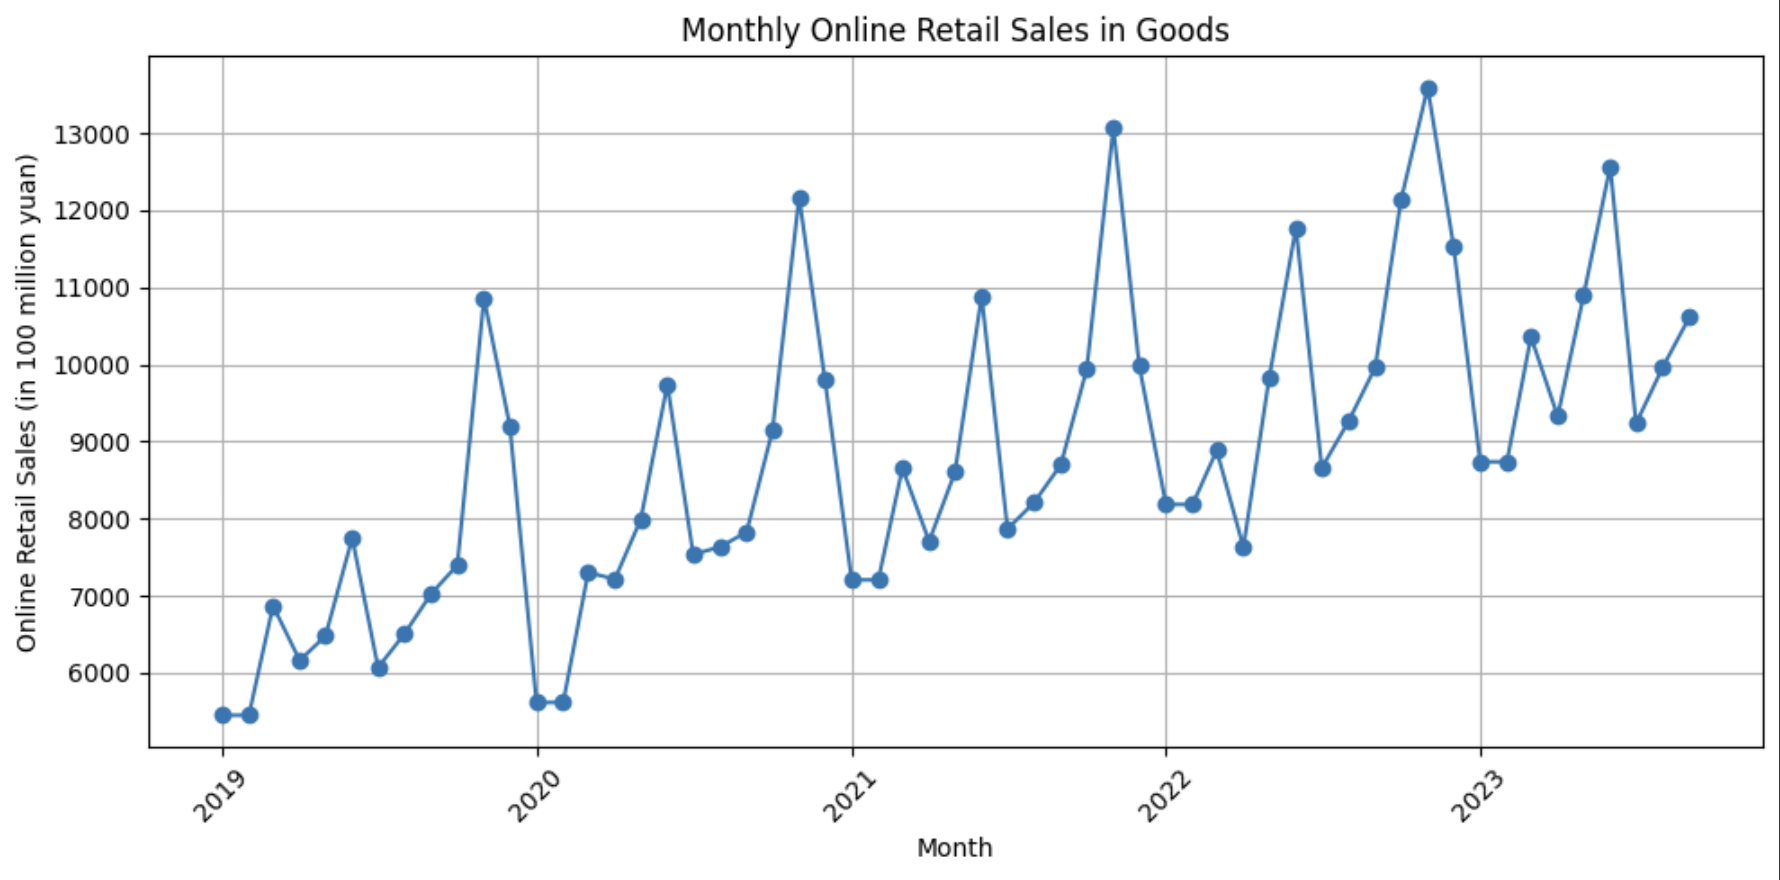
\includegraphics[width=0.8\textwidth]{online_sales_data.png}
  \caption{Online Sales Data}
  \label{fig:yourlabel}
\end{figure}

This graph represents monthly in-store retail sales in goods for the same time period.
The values here are also in millions and exhibit more significant fluctuations compared to the online sales data.
There seems to be a sharp increase or peak in sales around the start of 2020, which might indicate a seasonal effect or an event that caused an increase in in-store purchases.
Both graphs provide a visual representation of sales trends over time and could be useful for analyzing the performance of online vs. in-store sales, understanding seasonal effects on retail, and planning for inventory or marketing strategies.

\begin{figure}[h]
  \centering
  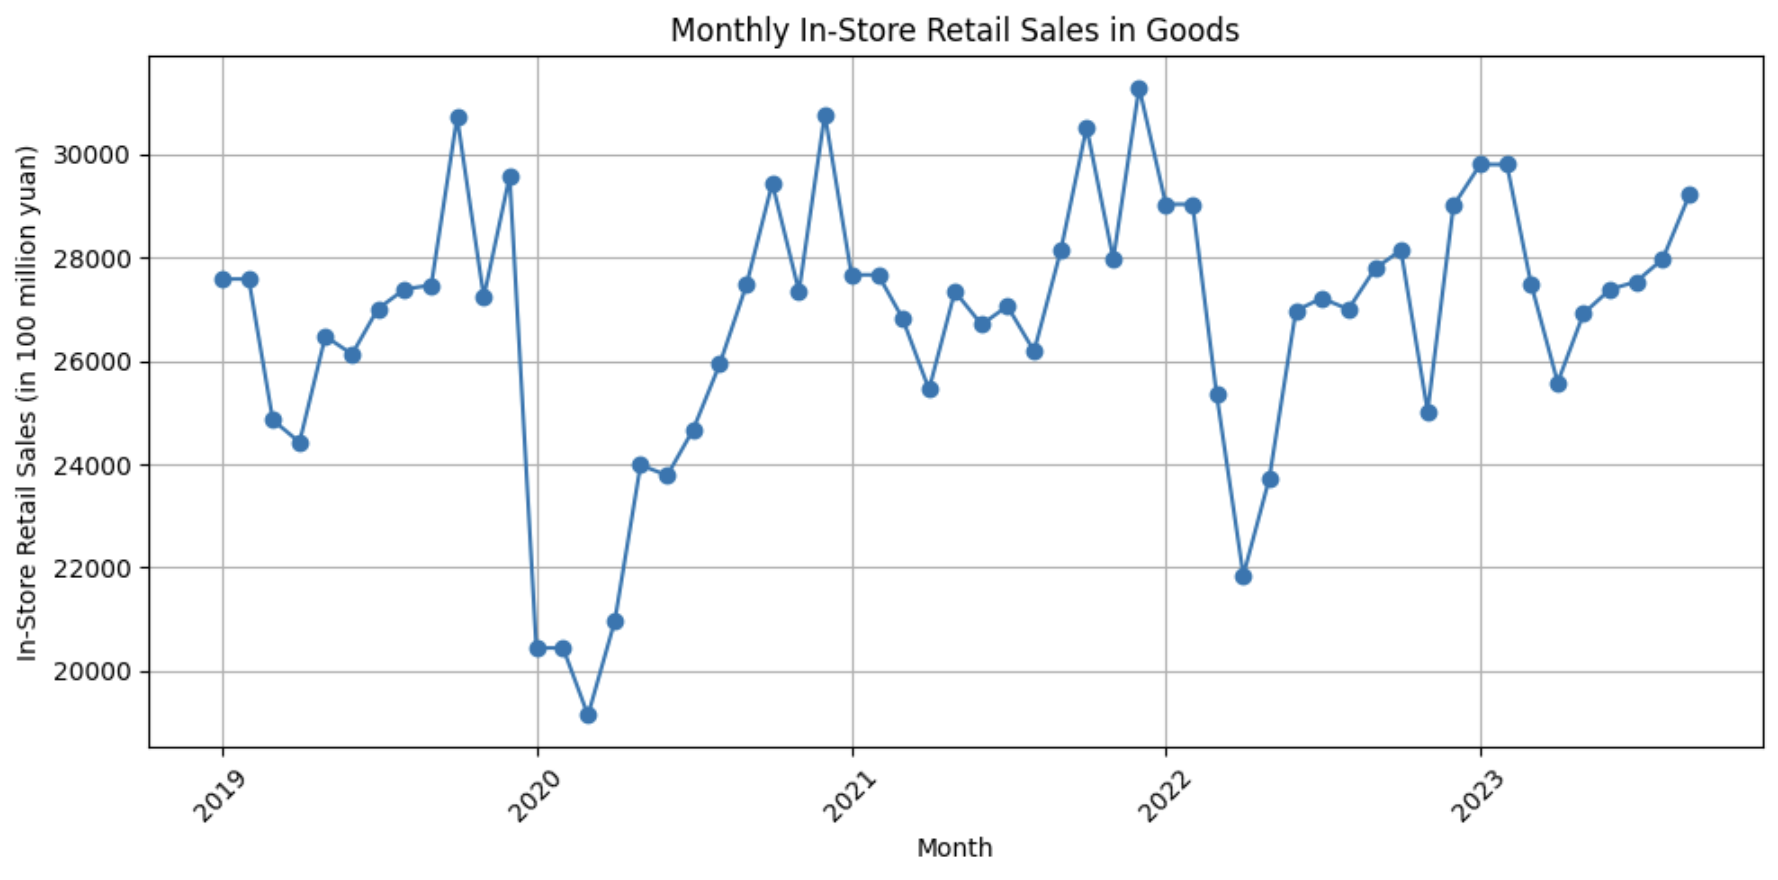
\includegraphics[width=0.8\textwidth]{offline_sales_data.png}
  \caption{Offline Sales Data}
  \label{fig:yourlabel}
\end{figure}


\begin{figure}[h]
  \centering
  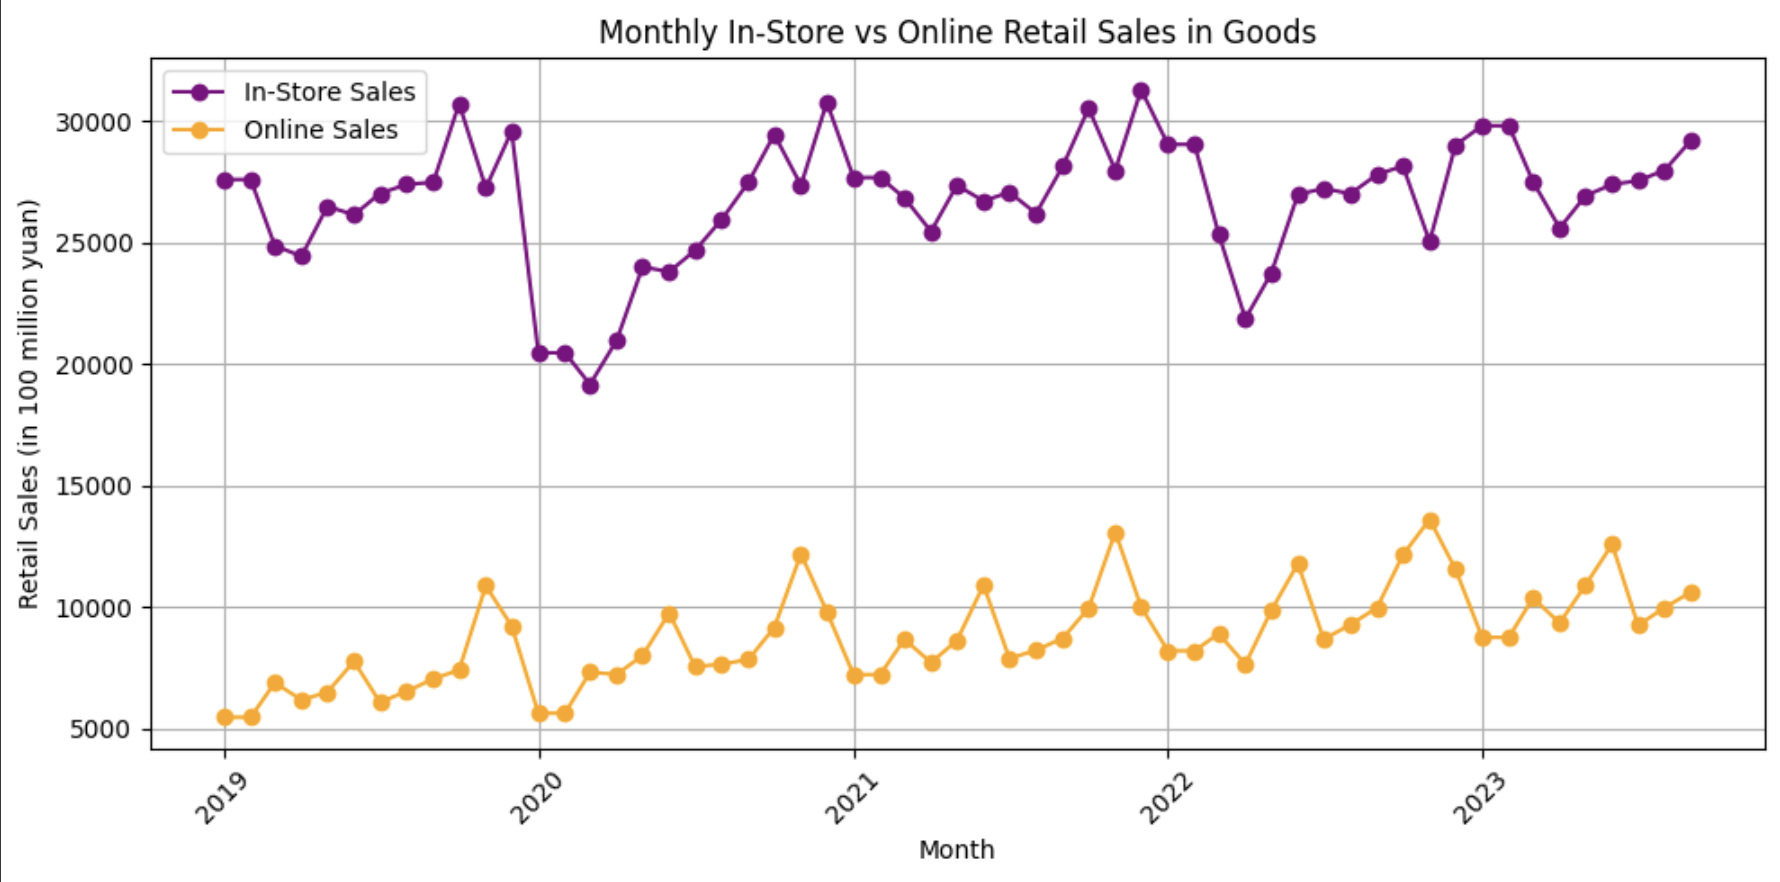
\includegraphics[width=0.8\textwidth]{online_offline_Compare.png}
  \caption{Online and offline sales compare}
  \label{fig:yourlabel}
\end{figure}


\section{Statistic analysis}
\subsection{Seasonal analysis}
\paragraph{Offline Seasonal analysis}
\begin{figure}[h]
  \centering
  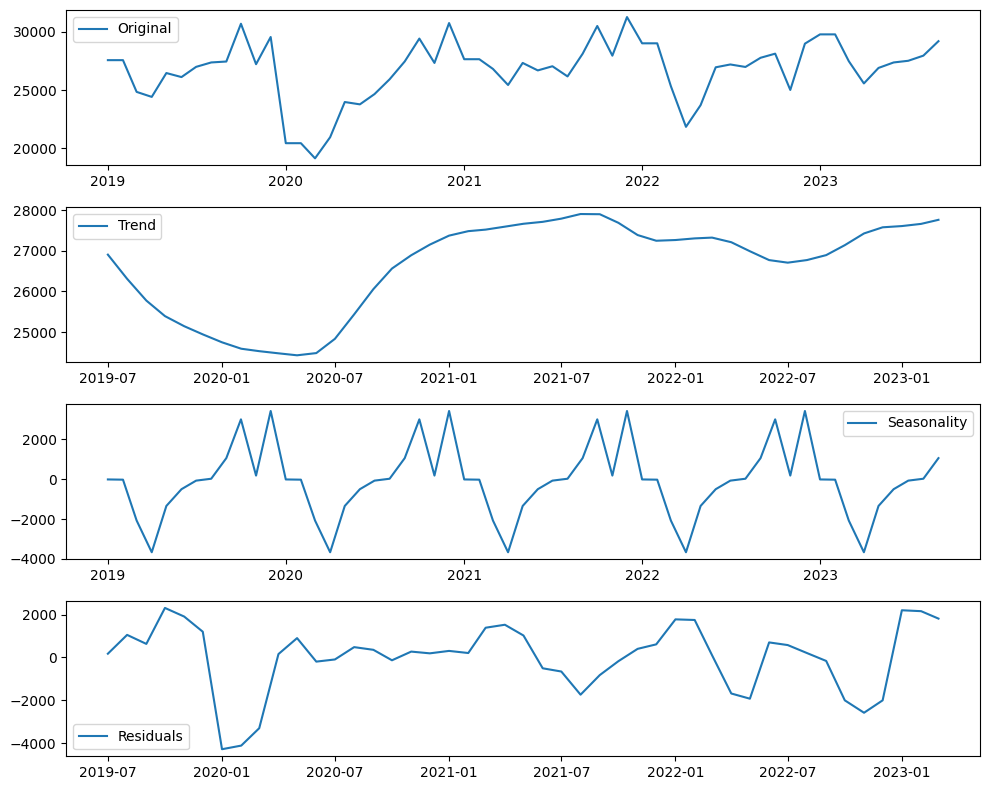
\includegraphics[width=0.7\textwidth]{Seasonal_analysis_offline.png}
  \caption{Offline Seasonal analysis}
  \label{fig:yourlabel}
\end{figure}

In Figure 4, Original Data shows the original monthly sales of physical store retail. From the figure we can see that sales show certain fluctuations, which may be caused by various factors such as market demand, promotional activities or seasonal factors.

The Trend section reveals the long-term trend of the data, eliminating the effects of seasonality and other irregularities. As can be observed from the chart, the trend line showed a decline at the beginning of 2020, which was most likely related to the COVID-19 pandemic, and then the data showed a gradual recovery and continued upward trend.

Seasonality reveals seasonal patterns in data, that is, regular fluctuations that occur periodically throughout the year. The chart indicates a regular increase or decrease in sales data during specific months, indicating that sales are significantly affected by seasonality.

\paragraph{Online Seasonal analysis}
\begin{figure}[h]
  \centering
  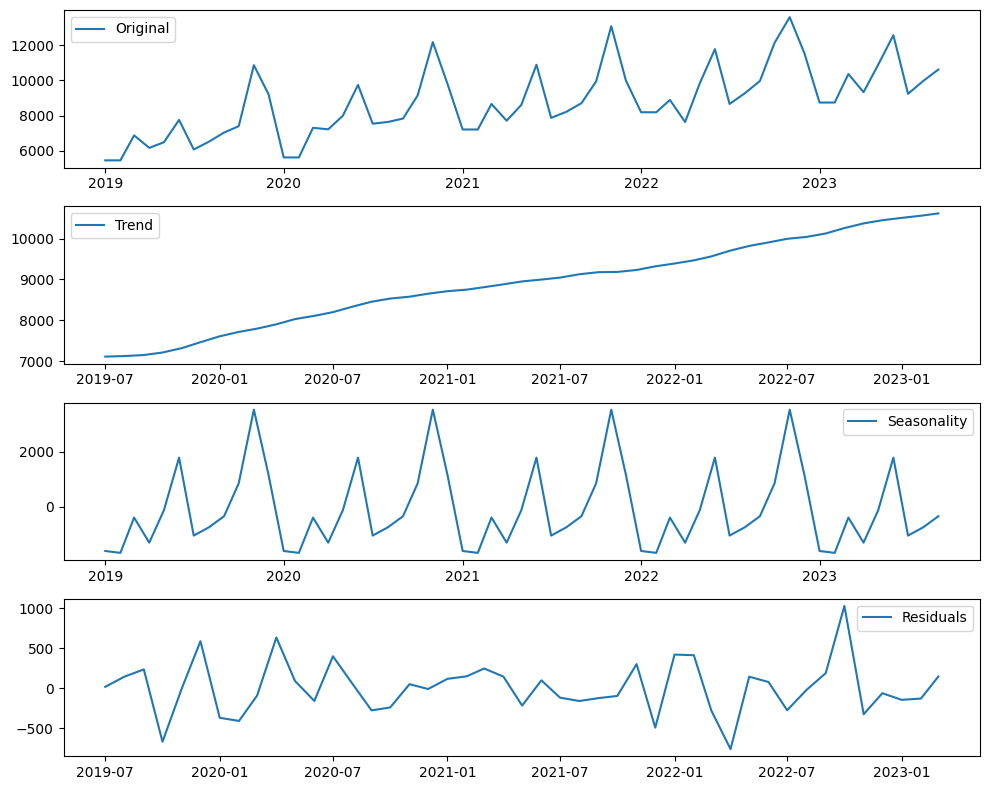
\includegraphics[width=0.7\textwidth]{Seasonal_analysis_online.png}
  \caption{Online Seasonal analysis}
  \label{fig:yourlabel}
\end{figure}

Figure 5 shows the patterns observed in online sales data over several years. The original data in the top chart captures the monthly fluctuations, showing peaks and troughs that reveal how online sales volumes change over time. Notably, there is an increase in sales towards the end of each year, likely influenced by annual e-commerce promotional events in November and December.
The trend component smooths out short-term irregularities and seasonal effects to elucidate the underlying long-term trend in online sales data. This trend is generally upward, indicating a consistent growth in online sales, which may be reflective of the broader expansion and adoption of e-commerce practices.

The seasonal component of the data illustrates the cyclic patterns that recur within each year. The regular occurrence of peaks and troughs suggests that online sales are significantly influenced by seasonal factors, such as holiday periods and specific sales events like Black Friday and Christmas, which traditionally see an uptick in retail activity. This seasonality is characteristic of the retail industry, where certain times of the year consistently exhibit higher or lower sales due to these well-established commercial and cultural events.

\subsection{t-test}
First, test the variance of the two sets of sample data: online monthly sales and offline monthly sales. At a significance level of 0.05, use the Levene statistic to determine whether the variances are equal based on the p value. If the p-value is less than the significance level, the variances of the two sets of data are considered to be unequal, and vice versa.
\\The results are shown as Levene Statistics: 0.6410067116098597, p -value: 0.42504157050096525
Therefore, we failed to reject the null hypothesis of equal variances and considered the variances of the two sets of data to be equal.
\\In the case of equal variances, We use t-test to test whether there is a statistically significant difference between the means of online and offline sales data.
\\Then, conduct a t test on the two sets of data, online monthly sales and offline monthly sales, to compare the means of sales. Choose a significance level of 0.05. If the test p-value is less than the significance level, the null hypothesis is rejected and there is no significant difference in the means of the two sets of sales data, and vice versa.
\\The results are displayed as t statistics: -41.477883180273004, p-value: 1.0659906776480866e-66. Therefore, we reject the null hypothesis and believe that there is a significant difference in the means of the two sets of data.

\subsection{Regression analysis}

\begin{figure}[h]
  \centering
  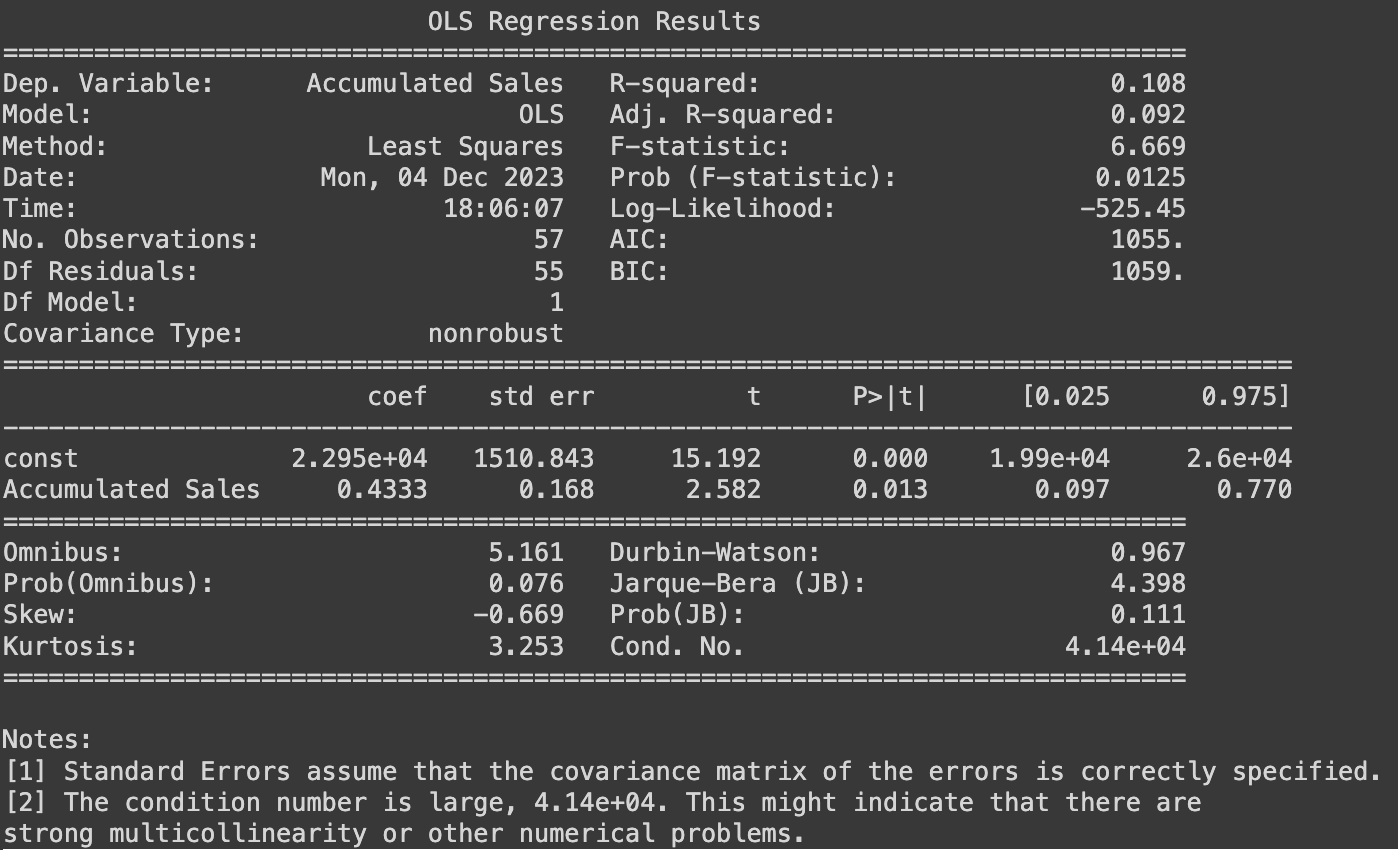
\includegraphics[width=0.8\textwidth]{Regression results.png}
  \caption{Regression results}
  \label{fig:yourlabel}
\end{figure}

The regression output provides various statistics about the relationship between online monthly sales (x) and in-store monthly sales (y).

The R-squared value is 0.108, meaning that approximately 10.8 of the variability in in-store sales can be explained by the variability in online sales. This is a relatively low value, suggesting that online sales are not a strong predictor of in-store sales.

The F-statistic is 6.669 with a p-value of 0.0125. This suggests that the model is statistically significant at a common alpha level of 0.05, meaning there is a statistically significant relationship between online and in-store sales.

Coefficients:
The intercept is approximately 22,950 with a p-value of 0.000, indicating that it is statistically significant. This value represents the expected in-store sales when online sales are zero.
The coefficient for online sales is 0.4333 with a p-value of 0.013, which is also statistically significant. This coefficient means that for every unit increase in online sales, in-store sales increase by approximately 0.4333 units.

In summary, while the model indicates a statistically significant relationship between online and in-store sales, the low R-squared value means that online sales are not a strong predictor of in-store sales. With the growth of online retail sales, the in-store retail sales will also increase slightly.

This is contrary to our guess that the growth of online sales will greatly weaken offline sales. The reason for this may be that the overall social economy has recovered after the epidemic, and both online and offline sales have increased.

\subsection{Deseasonalized regression}

\begin{figure}[h]
  \centering
  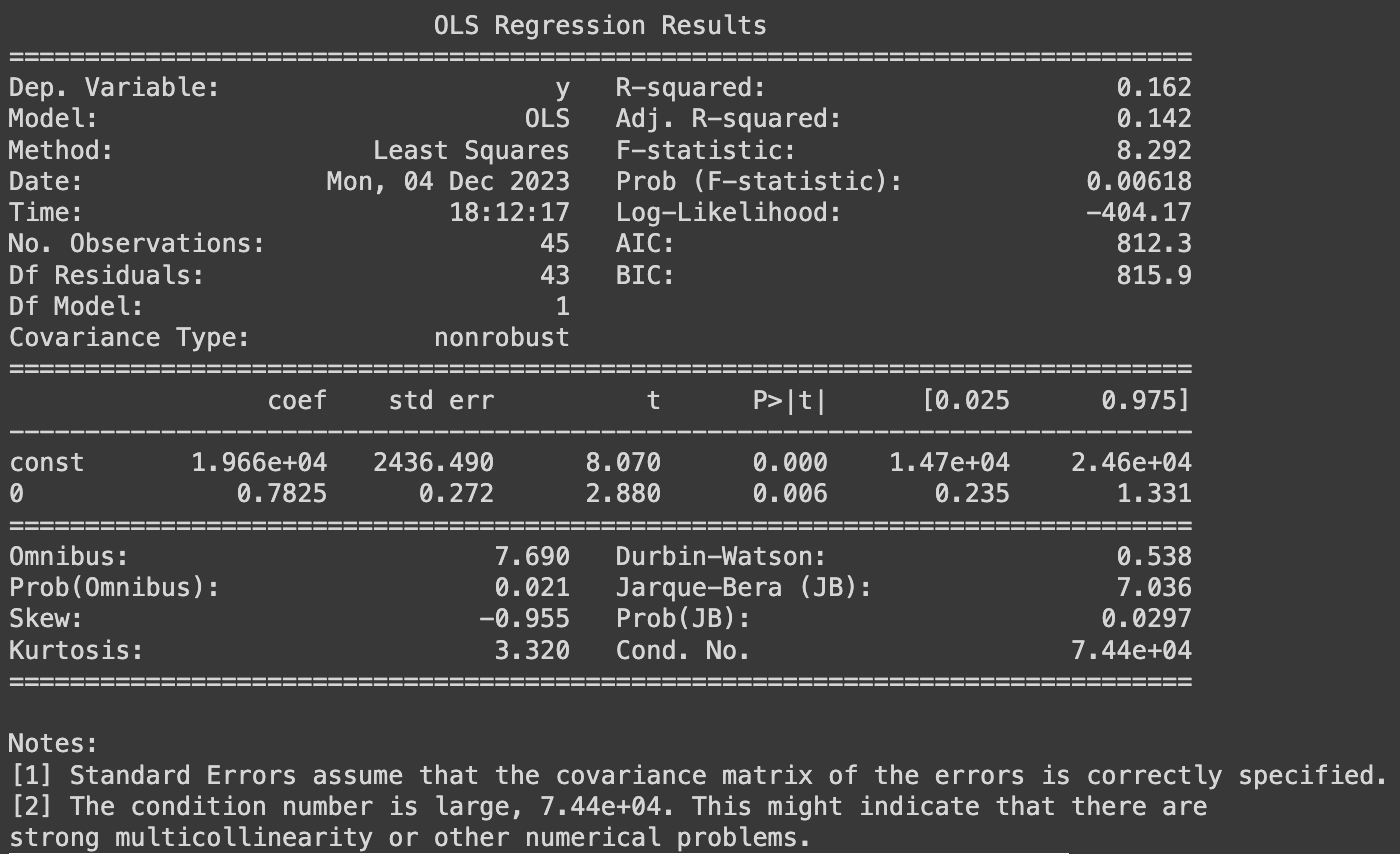
\includegraphics[width=0.8\textwidth]{Deseasonalized regression.png}
  \caption{Regression results}
  \label{fig:yourlabel}
\end{figure}

After removing the seasonality factor and performing the regression analysis, here's the interpretation of the results:

The R-squared value is 0.162, which indicates that the model explains 16.2 of the variance in the de-seasonalized in-store sales. This is an improvement over the previous model with seasonality, suggesting that online sales are a more significant predictor of in-store sales after removing the seasonal effect.

The F-statistic is 8.292 with a p-value of 0.00618. This suggests that the model is statistically significant, and the relationship between online sales and de-seasonalized in-store sales is not due to random chance.

The coefficient for the constant term is approximately 196,600 with a p-value close to 0. This suggests a significant intercept, which could be interpreted as the baseline level of in-store sales when online sales are zero (assuming the model is correctly specified).

The coefficient for online sales is about 0.7825 with a p-value of 0.006, indicating a statistically significant relationship between online sales and de-seasonalized in-store sales. For every unit increase in online sales, de-seasonalized in-store sales increase by approximately 0.7825 units.

\section{Conclusion}

\newpage
\bibliographystyle{alpha}
\bibliography{sample}

\end{document}


@article{luo2019commerce,
  title={E-Commerce development and household consumption growth in China},
  author={Luo, Xubei and Wang, Yue and Zhang, Xiaobo},
  journal={World Bank Policy Research Working Paper},
  number={8810},
  year={2019}
}
@article{luo2019commerce,
  title={E-Commerce development and household consumption growth in China},
  author={Luo, Xubei and Wang, Yue and Zhang, Xiaobo},
  journal={World Bank Policy Research Working Paper},
  number={8810},
  year={2019}
}